%!TEX root = ../dokumentation.tex

\chapter{Theory}\label{cha:Theory}

\section{Orchestration and Choreography}\label{cha:Theory:orchestrationchoreography}

In a microservice architecture, there are mainly two patterns for service communication, namely orchestration or choreography.
For choreographed systems, synchronous messaging is commonly used.
With synchronous messaging, the communication follows a request-response pattern, where the caller expects an immediate answer, thus also called blocking messaging.
Each service communicates directly with the other service, without needing intermediary services such as a broker, as seen in Figure \ref{img:choreographedCommunication}.
Consequently, choreographed communication has a very low latency and high performance for point to point communication.
However, a broker-less design results in services either having to know the location of a service or they need to rely on a service discovery \cite{NoorainPanjwani.2020}\cite{Rudrabhatla.2018}.
\begin{figure}[h]
	\centering
	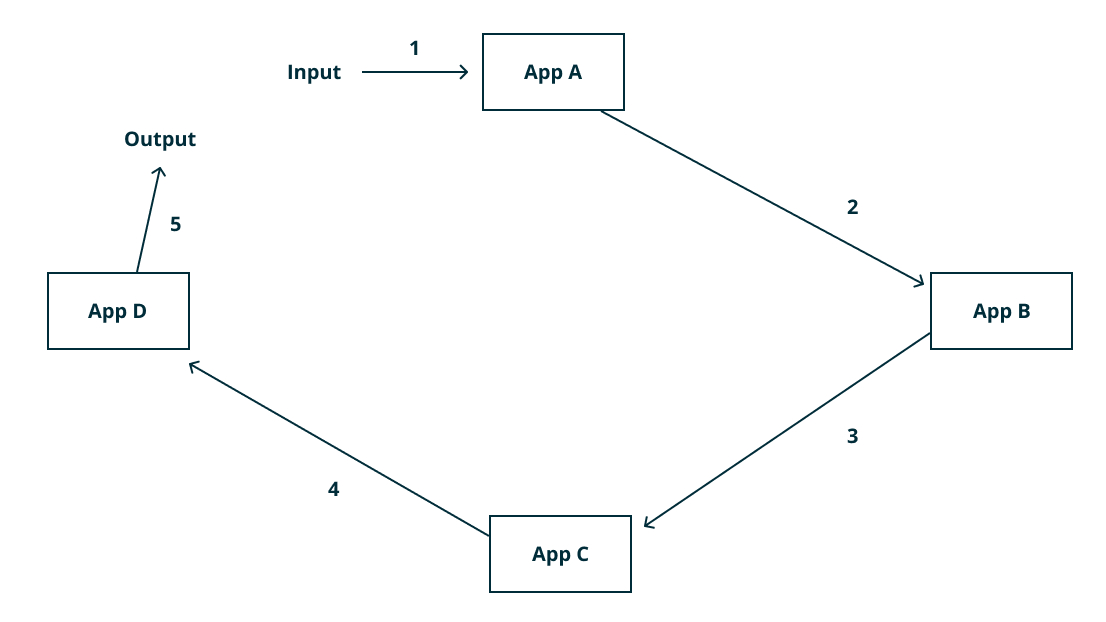
\includegraphics[width=\textwidth, height=0.5\textheight, keepaspectratio]{brokerless.jpeg}
	\caption{Choreographed communication architecture \cite{NoorainPanjwani.2020}}
	\label{img:choreographedCommunication}
\end{figure}

On the other hand, orchestrated architectures need brokers, to which the services connect to.
This eliminates the need for a service discovery, as services are completely decoupled from each other and are more flexible with an asynchronous messaging system (cf. chapter \ref{cha:Theory:async}).
An exemplary flow of communication can be seen in Figure \ref{img:orchestratedCommunication}, where apps/services communicate only over a broker and do not necessarily need a response to a message (e.g \textit{App C}).
The latter case could be a monitoring service, which only collects metrics.
Having a intermediary service, however, always results in a higher latency and higher resource utilization, as compared to direct synchronous communication.
Consequently, broker-based architectures are used over broker-less designs with service discovery in cases, where the benefits such as queueing or broadcasting can be leveraged \cite{Rudrabhatla.2018}\cite{Giro.2019}.

\begin{figure}[h]
	\centering
	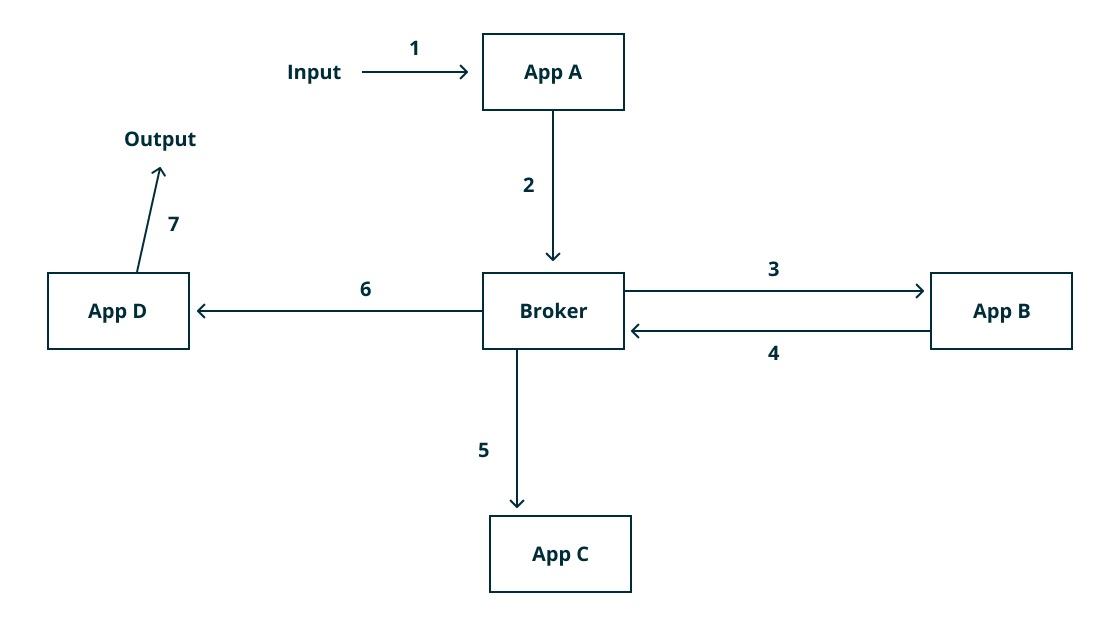
\includegraphics[width=\textwidth, height=0.5\textheight, keepaspectratio]{brokerbased.jpg}
	\caption{Orchestrated communication architecture \cite{NoorainPanjwani.2020}}
	\label{img:orchestratedCommunication}
\end{figure}

\section{Asynchronous messaging}\label{cha:Theory:async}

Asynchronous messaging is used to provide a flexible communication channel between clients.
In such an environment, transferred messages are called events.
As shown in Figure \ref{img:asyncMessagignPrincipal}, a client can either produce or consume events.
To transfer an event, typically a \textit{broker} is needed, which is part of an independent system.
Therefore, the communication flow can be described as follows:
The producer client sends an event to a \textit{broker}, which then routes the event to a consumer client.
Depending on the used \textit{broker}, the available routing mechanisms change.
Routing is an important part of asynchronous messaging \cite[p.~62f.]{Bruce.2019}.

\begin{figure}[h]
	\centering
	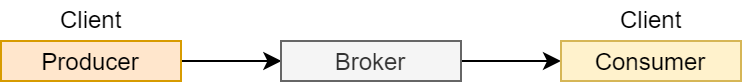
\includegraphics[width=\textwidth, height=0.9\textheight, keepaspectratio]{theorie_async_messaging.png}
	\caption{Asynchronous messaging principal}
	\label{img:asyncMessagignPrincipal}
\end{figure}

Most higher level interaction patterns for asynchronous messaging are based either on the \textit{job queue} or \textit{publish-subscribe} pattern.
The concept of a \textit{job queue} is to distribute work via events to consumers.
To allow this behavior, the \textit{job queue} provides a queue, where producers can send their events to.
Consumers then consume these events, thus emptying the queue.
It is important to note, that not every consumer receives every event.

An example for the \textit{job queue} is shown in Figure \ref{img:asyncJobQueue}.
In this example, an \textit{Order} service creates orders and two \textit{Market} services pickup the events and process them.
As already pointed out, events are not duplicated and hence only one service can consume them \cite[p.~63f.]{Bruce.2019}.

\begin{figure}
	\centering
	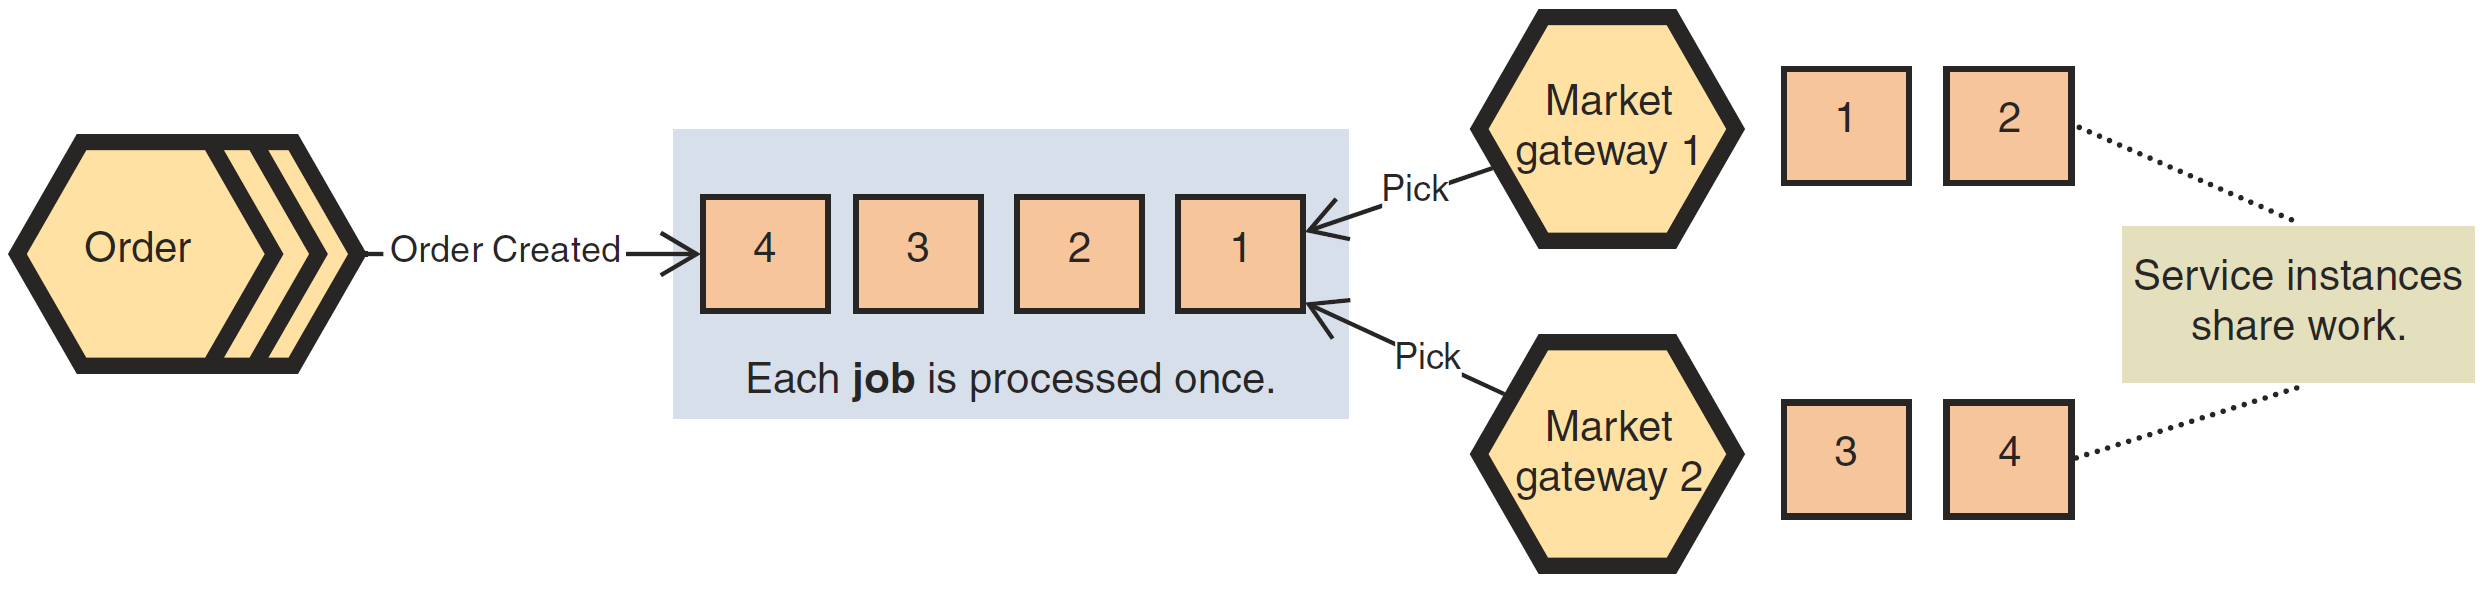
\includegraphics[width=\textwidth, height=0.9\textheight, keepaspectratio]{theorie_async_jobqueue.png}
	\caption{Asynchronous communication pattern job queue example \cite[p.~64]{Bruce.2019}}
	\label{img:asyncJobQueue}
\end{figure}

The second common pattern is the \textit{publish-subscribe} pattern, which is especially important for this work.
The concept of \textit{publish-subscribe} is to inform arbitrary listeners about something.
As the name implies, a client can publish an event which listeners (\textit{subscribers}) receive.
In this case, each event is distributed to each subscriber.
An example for the \textit{publish-subscribe} is shown in Figure \ref{img:asyncPubSub}.
There, a service \textit{Market} publishes the event \textit{oder placed}, which services like \textit{Notify} and \textit{Statistics} subscribe to.
Consequently, all the subscribers receive the event \cite[p.~64f.]{Bruce.2019}.

\begin{figure}
	\centering
	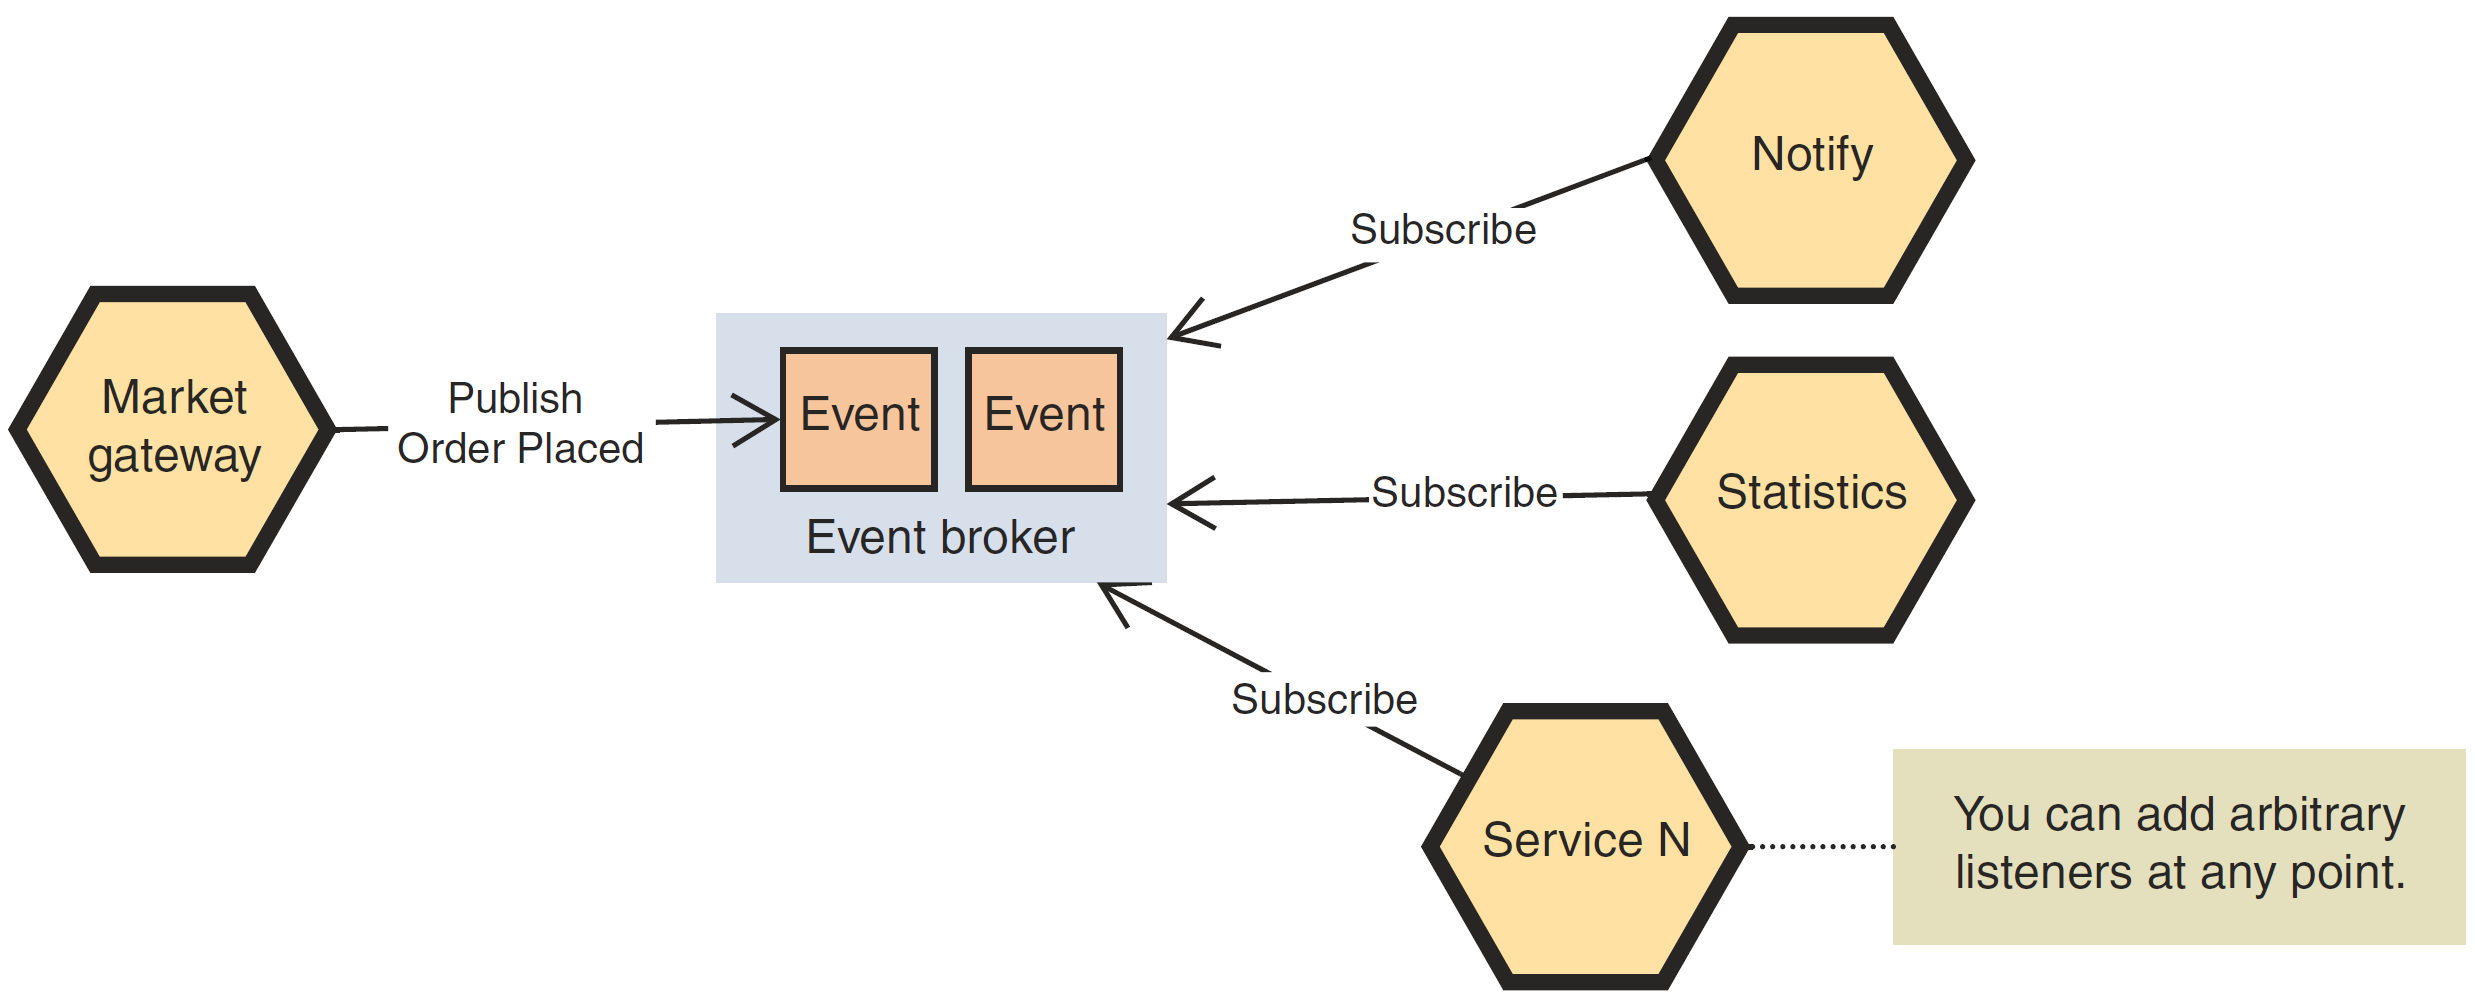
\includegraphics[width=\textwidth, height=0.9\textheight, keepaspectratio]{theorie_async_pubsub.png}
	\caption{Asynchronous communication pattern publish-subscribe example \cite[p.~64]{Bruce.2019}}
	\label{img:asyncPubSub}
\end{figure}

Another important aspect to consider when working with asynchronous messaging are the delivery guarantees.
In the context of the \acf{MQTT} protocol this is called \acf{QoS}.
There are three level of \ac{QoS}, \textit{at-most-once}, \textit{at-least-once} and \textit{exactly-once}.
All levels target the consumer and how events are received in a case of a failure \cite[p.~59f.]{Aziz.08.09.201412.09.2014}\cite{AndrewBanks.2014}.
\begin{itemize}
	\item \textit{at-most-once}: The consumer receives an event once or not at all.
	\item \textit{at-least-once}: The consumer is guaranteed to receive the event, but it could receive the same event more than once.
	\item \textit{exactly-once}: The consumer receives an event exactly once.
\end{itemize}

These \ac{QoS} levels are also applicable to other protocols or technologies.